\documentclass[licenciatura]{unb-cic}
\usepackage[american,brazil]{babel}
\usepackage[T1]{fontenc}
\usepackage{indentfirst}
\usepackage{natbib}
\usepackage{xcolor,graphicx,url}
\usepackage[utf8]{inputenc}

\bibpunct[; ]{(}{)}{,}{a}{}{;}%muda colchetes para parênteses

% definições prévias do documento
\title{Sintese de Voz}

\orientador{\prof \dr Jorge Carlos Lucero}{CIC/UnB}

\coordenador{\prof \dr Coordenador}{CIC/UnB}

\diamesano{10}{maio}{2016}

                           
\membrobanca{\prof\dr Professor I}{CIC/UnB}

\membrobanca{\prof \dr Professor II}{CIC/UnB}

\autor{Leandro Ramalho Motta}{Ferreira}
\CDU{004.4}

\palavraschave{Sintese, Voz, Saúde}
\keywords{Synthesis, Voice, Health}


\begin{document}

\maketitle

\pretextual
\begin{dedicatoria}
Dedico a....
\end{dedicatoria}

\begin{agradecimentos}
Agradeço a....
\end{agradecimentos}

\begin{resumo}
AINDA Não tem

\end{resumo}

\selectlanguage{american}

\begin{abstract}
Still there isn't.
\end{abstract}

\selectlanguage{brazil}
\tableofcontents
\listoffigures
\listoftables

\textual


\chapter{Introdução}

	\section{Motivação}
		A UnB possúi atuação na área de simulação de voz a ser considerada. Essa atuação considero ser principalmente ser por esforço e trabalho do Doutor Jorge Carlos Lúcero do Departamento de Ciência da Computação. Seu trabalho de simulação de voz e simulação de voz com patologias na área da saúde precisa ter um apoio. Este Trabalho de conclusão de curso é feito com intuito de seguir uma nova direção na área de simulação de voz mas mantendo os avanços já feitos por outros trabalhos, sendo essa direção nova a do entretenimento.
		
		Mercadológicamente a música é um campo muito interessante economicamente, onde produtos da área de síntese de voz estão cada vez mais avançados, por exemplo o sucesso das Vocaloids no japão. Por outro lado sintetizar vozes e a área de música são atualmente meu sonho de projeto.

\chapter{Conceitos Básicos de Sintese de Voz}
\section{Anatomia da Voz}
	Para estudar a produção e a síntese da voz, é necessário ter um conhecimento acerca da anatomia e do funcionamento físico da voz \citenum{Foundation1}. Sendo assim, as subseções seguintes descreverão brevemente detalhes da anatomia do sistema fonador humano e como o som é produzido, moldado e influenciado por este sistema.
	
	\begin{figure}
		\centering
		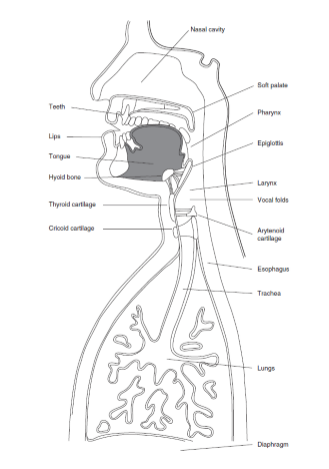
\includegraphics[scale=0.5]{aparelhoFonador}
		\caption{Aparelho Fonador}
		\label{fig:aparelhoFonador}
	\end{figure}
	\subsection{Aparelho Fonador}
	O estudo do aparelho fonador começa-se por suas estruturas e componentes importantes. Após um estudo detalhado dos fenômenos físicos e como se comportam é essencial também.
		
	A Figura \ref{fig:aparelhoFonador} \citenum{Foundation1}, mostra os órgãos associados com a produção da voz. 
	
	Dentro das condições normais, a voz é produzida quando um fluxo de ar vindo dos pulmões é convertido em energia acústica através da vibração das pregas vocais, localizadas na laringe. Os padrões de vibrações resultantes são moldados acusticamente quando o som passa pelo trato vocal acima da laringe. O sistema respiratório serve como uma
	fonte de potência para a produção do som, sendo responsável por movimentar o ar através do trato vocal. A laringe atua como um oscilador convertendo a potência aerodinâmica produzida em energia sonora, sendo frequentemente retratada como a fonte da voz. No entanto, a mais importante função da laringe não é a produção de som, e sim, vedar as vias aéreas aos pulmões completamente, protegendo-as de objetos estranhos ou líquidos, principalmente durante a deglutinação. De maneira análoga, a laringe serve como uma válvula de acesso às vias respiratórias e por essa característica, atua também no controle do fluxo de ar que por elas passam. Sendo assim,é fácil notar que há uma necessidade de mobilidade para toda estruturada laringe, logo é de se esperar que sua estrutura seja formada em sua maioria por cartilagens. De fato o é, com exceção de um osso chamado de Hioide, a laringe é basicamente formada por cartilagens e músculos. A seguir, analisaremos brevemente a dinâmica dos músculos e cartilagens da laringe.
	
\subsection{Músculos e Cartilagens}
Os músculos e cartilagens atuam diretamente no processo de abdução e adução das pregas vocais. Estas estão localizadas dentro da laringe e devido à dinâmica das cartilagens e dos músculos, podem executar os movimentos citados de forma a produzir som.

\subsubsection{Cartilagens da Laringe }
\begin{figure}
	\centering
	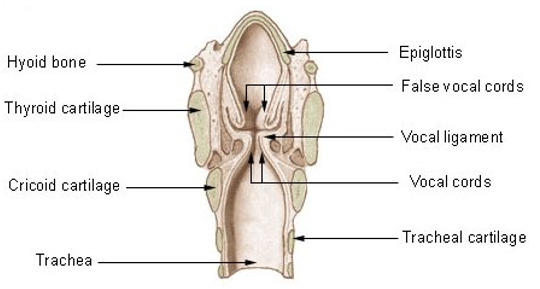
\includegraphics[scale=0.5]{musculosCartilagens}
	\caption{Secção coronal da laringe e parte superior da traquéia}
	\label{fig:Cartilagens}
\end{figure}
A Figura \ref{fig:Cartilagens}, mostra uma secção da laringe, detalhando as cartilagens presentes.
De maneira sucinta, estas cartilagens servem como base de interconexão para os músculos intrínsecos ao redor da laringe. Dentre as cartilagens acima, a epiglote é responsável por vedar as vias respiratórias movimentando-se sobre a entrada das mesmas. O resto das cartilagens garantem a mobilidade da laringe em conjunto com outras estruturas como por exemplo o sternum.


\subsubsection{Músculos da Laringe}
Os músculos na laringe podem ser divididos em dois grupos, os intrínsecos e os extrínsecos \citealp{Giovanni20041}. Os músculos intrínsecos interconectam as cartilagens da laringe, ao passo que, os extrínsecos conectam a laringe à outras estruturas externas, como o osso hióide. A Figura \ref*{fig:musculos} detalha alguns dos músculos intrínsecos da laringe. Alguns desses músculos têm influência direta em algumas características da voz. Por exemplo, o músculo cricotiroideo é o músculo primário utilizado no controle do tom da voz. Por sua vez, o músculo cricoaritenoideo posterior atua na abdução das pregas vocais, ao passo que o músculo interaritenoideo atua como adutor das pregas vocais.

\begin{figure}
	\centering
	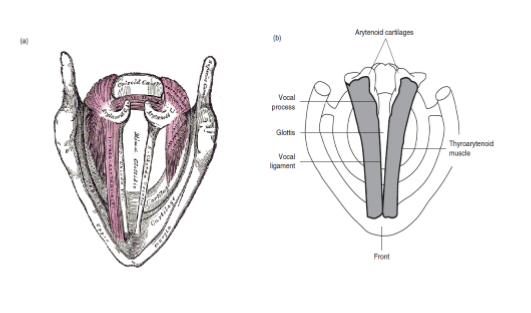
\includegraphics[scale=0.5]{musculosLaringe}
	\caption{Músculos Intrínsecos da Laringe}
	\label{fig:musculos}
\end{figure}

Os músculos extrínsecos, Figura \ref{fig:musculoExterno}, atuam basicamente no movimento da laringe, agindo como depressor e elevador da estrutura laríngea. Além disso também conectam estruturas do trato vocal à estrutura laríngea, como por exemplo a língua ao osso hioide.


\begin{figure}
	\centering
	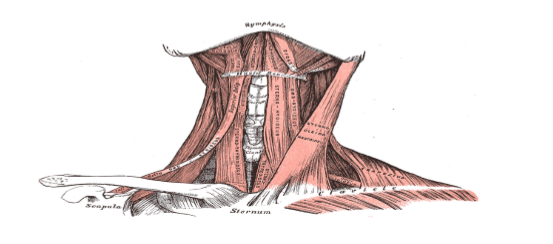
\includegraphics[scale=0.5]{musculosExternosLaringe}
	\caption{Músculos Extrínsecos da Laringe }
	\label{fig:musculoExterno}
\end{figure}

\subsection{Pregas Vocais}

As pregas vocais, como dito anteriormente, estão localizadas dentro da laringe, mais específicamente na parte superior da traqueia. Elas estão posteriormente ligadas às cartilagens aritenoides, e anteriormente ligadas à cartilagem tireoide. As suas bordas exteriores estão ligadas a músculos na laringe, enquanto as suas bordas interiores são livres.

As bordas das pregas vocais são construídas de epitélio, sendo compostas também de algumas fibras musculares. As pregas vocais são bandas triangulares planas de cor branca e acima de ambos os lados destas, se encontram as pregas vestibulares ou falsas pregas vocais. 

O espaço entre as pregas vocais é chamado de glote, sendo que o que está acima da glote é denominado supraglotal e o que está abaixo é denominado subglotal. A Figura 1.5 mostra em mais detalhes a anatomia das pregas vocais, os componentes musculares e as cartilagens atuantes.

\begin{figure}
	\centering
	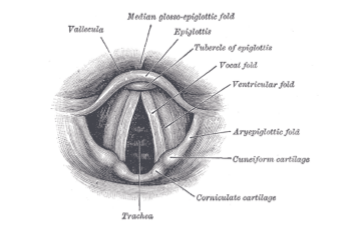
\includegraphics[scale=0.5]{cordasVocais}
	\caption{ Cordas Vocais e Componentes}
	\label{fig:cordasVocasi}
\end{figure}

\section{Propriedades Físicas}

	\subsection{Lei Bernouli}
		Energia potencial e energica cinética em fluídos se mantém a mesma
		porém em proporções diferentes \cite{BradhStory}:
		
		\[
		P + \frac{\rho * v^2}{2} = Constante\\
		Sendo: \\
		\rho = Densidade do fluido \\
		P = Pressão no duto onde o fluído se encontra\\
		v =  velocidade da particula 
		\]
	\subsection{Critérios para Oscilação}
		Alguns critérios devem ser atendidos para que um determinador padrão de movimento seja considerado como uma oscilação mecânica, a saber:
		
		
		No sistema onde ocorre o movimento deve haver uma posição de equilíbrio estável, que é caracterizada por uma força restaurativa que sempre acelera o corpo em	movimento de volta para a sua posição de repouso.
		Deve haver inércia(no caso do sistema mecânico, a massa atua como propriedade de inércia) no sistema para superar esta posição de equilíbrio.
		A perda, em excesso, de energia por ciclo de oscilação deve ser zero.\ldots 
	
	\subsection{Tipos de Oscilação}
			De acordo com Titze~\cite{IngoTitze}, os tipos de oscilação são:
			\begin{itemize}
				\item  Oscilação Natural: Quando um sistema que se encaixa nos critérios anteriores se move sem interferência após um distúrbio inicial.
				\item Oscilação Natural: Quando um sistema que se encaixa nos critérios anteriores se move sem interferência após um distúrbio inicial.
				\item Oscilação Forçada: Requer uma fonte externa de condução que por si só é um
				oscilador. Dita grande parte do padrão de vibração do sistema.
				\item Oscilação Auto-Sustentável: Requer uma fonte de energia estável e uma interação não-linear entre os componentes internos ao sistema. As perdas de energia são compensadas, mantendo o padrão oscilatório.
			\end{itemize}
		
	\subsection{Tensao}
		Conceito de Tensão For por unidade de ar
		
		\[
		\sigma = \frac{F}{A}
		\]
		Sendo:
		f : força aplicada. \linebreak
		A: área de aplicação desta força.
		
	\subsection{Curva Força e Alongamento}
		Utiliza-se para não ser dependente da geometria do material. Utilizamos nas cordas vocais(?) por serem materias biológicos. Cria uma figura ilustrando comportamento da deformação das pregas vocais
		
		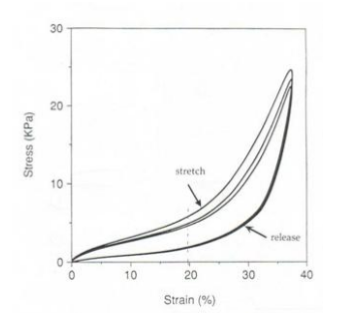
\includegraphics{figura1.png}
		
	\subsection{Viscosidade}
		É a velocidade de deformação(consequentemente, de restauração) de
		um determinado fluido quando atuam forças de tensão no mesmo. Matematicamente
		pode ser expresso conforme a equação seguinte: \citenum{Ingo}
		
		$
		\sigma = \eta * \frac{d*\epsilon}{dt}
		$
		
	
	\subsection{Reflexao de Som}
	
		Um fenômeno ligado a rigidez e amortecimento entre um meio e outro.\cite{MTAGENTE}
		Ondas quando tentam penetrar em um segundo meio, sendo o segundo meio rígido, as partículas primeiro meio se aglomeram tentando passar porém
		falham, seu acúmulo de particulas geram pressão que acabam criando uma outra onda no primeiro meio decorrente da primeira onda.\cite{HenryGray}
		
		O mesmo ocorre com o meio 2 sendo totalmente não rígido e o primeiro meio sendo bem rígido, Exaurindo excesso de particulas  do meio 1 no meio 2 criando rarefação no meio 1, o que cria uma outra onda de pressão negativa~\cite{FlanaganLandgraf}. A propagação é sempre em direção oposta à fonte, no caso é na direção contrária à coluna de ar(meio 1). 
	
	
	\subsection{Fluxo de Ar na Glote}
	
		Fluxo de ar na Glote:
		
		Como descrito no artigo de Elias temos informações como descobrimos a pressão via fluxo de ar\cite{eliasamadeudesouza}
	
		\[
		U_g = +-(\frac{-a_m}{A_*}+[(a_m)^2 +- (\frac{4K_t}{C^2\rho})](P^+_s - P^-_i))
		\]
		
		\[
$		A^*  = \text{Área efetiva computada pelas areas A_i e A_s}$
		\]
		
		\[
$		\rho = \text{Densidade do Ar}$
		\]
		\[
$		c = \text{Velocidade do som}$
		\]
		
		\[
$		P_s e P_i = \text{Pressão de incidencia na entra e saída da glote}$
		\]
		
		Uma vez descoberto o fluxo, as pressões de reflexão P^s_ e P^+_i podem ser encontradas com a seguinte equação:
		
		\[
		P^-_s = P^+_s - (\rho c / A_s) U_g
		\]
		
		
		\[
		P^+_i = P^-_i - (\rho c / A_i) U_g
		\]
		
		Quando ocorre o fechamento da glote então alguns parametros assumem valores conhecidos. a(t) = 0 , 
		$P_g = \frac{P_s-P_i}{2}$ e $U_g = 0$	
	
	
		





\section{Sintetizadores de Voz}
	\subsection{Modelo Massa-Mola Auto Sustentável}:
	A fechadura e abertura da glote num sistema massa mola de apenas um lado

	\[
		P = (1 - \frac{a2}{a1})*(Ps- Pi) + Pi
	\]
		
	
	Versão simplificada da pressão massa mola
	\begin{itemize}
		\item P: Pressão resultante NA GLOTE
		\item a1: Areas de entrada da glote
		\item a2: Areas de saída  da glote
		\item Ps: Pressão subglotica
		\item Pi: Pressão sobre o trato vocal(Pressão input)
	\end{itemize}
	
		No modelo mono massa a1 = a2.No caso em que Pressão na GLOTE,P, seja  igual a pressão  supraglotal, indica que a inércia da coluna de ar acima da glote altera a pressão.
	
	
	\subsection{Synpath}
		Sintetizador computacional, criado por Lucero.Sintetizador concebido por Fraj \cite{JeanFrancis}
		Foi escolhido não usar o modelo multi-massa por variações não suaves  e é tematicamente muito complexo apesar instabilidades numéricas.
		Synpath utiliza como base de representação das pregas vocais o modelo mono massa. O trato vocal é representado por uma concatenação de tubos cilindricos os quais se propagam uma onda acustica.Superglótica não leva em conta o trato vocal.Perdas e viscosidade são considerada.
	
		\subsubsection{Requisitos Funcionais}
		
		O Synpath é consistido também dos seguintes requisitos funcionais, os requistos funcionais são as funcionalidades que o sistema executará\cite{SWEBOK}
		
		\begin{itemize}
			\item 1 - Validação do Parâmetros passados pelo Usuário, se condizem com restrições do programa.
			\item 2 - Plotar um gráfico inicial do trato vocal de acordo com os parâmetros do usuário.
			\item 3 - Plotar três gráficos referentes as propriedades da voz simuladas com os parâmetros fornecidos pelo usuário. – O primeiro gráfico refere-se às posições adotadas pelas cordas vocais, a área da glótis, ao fluxo de ar nessa área e às características desse fluxo. – O segundo gráfico refere-se às características do som gerado pela simulação física do aparato fonador pelo programa. – O terceiro gráfico refere-se ao espectro de frequência do som gerado e do fluxo da glótis.
			\item 4 - Gerar um arquivo de texo com as características de voz gerada, frequencia,amplitude, ruído da voz, entre outros
			\item 5 Gerar um arquivo de som de voz simulada.
		\end{itemize}
		
		\subsubsection{Requisito Não-Funcionais}
		
		O Synpath consiste também dos seguintes requisitos não funcionais, requisitos não funcionais são requisitos são parametros de qualidade, requisitos que limitam as funcionalidades do sistema\cite{SWEBOK}.
		
		\begin{itemize}
			\item 1 - O Sistema deve produzir os gráficos que os requisitos funcionais delimitaram em um intervalo de 1(um) minuto. 
			\item 2  - Após gerar os gráficos e os exibi-los o arquivo texto e o arquivo de audio deverão ser exibidos
			\item 3 - Para que o sistema esteja funcional é necessário ter instalado os pacotes: MatPlotLib e NumPY
			\item 4 - O sistema deve ser executado em plataformas de um sistema operacionais como Windows, Linux ou MacOs, Versões recentes de acordo com a data desse documento. 
			
		\end{itemize}
		
	
	
	\subsection{HMMs}
		Minera-se de várias partituras musicais para treino. Os dados minerados dessas músicas são fonemas, altura, intensidade e os intervalos, isto é relação com outras notas.Esses dados são convertidos e mapeados em "labels" dependentes de contexto~\cite{DegottexNada}.Após isso as HMM's são treinados através dos dados de treinamento usando o algoritmo EM.\cite{GudnasonNada}. Após isso ocorre a fase de sintesis, usa-se outra partitura para ser convertida em "labels" dependentes de contexto e estima-se quais "labels" preprocessadas são correspondentes.\cite{TakashiNose}
	
		\subsection{MHRSMM}
		Uma variação HSMM. Modelo de multipla regressão HSMM.
		Parametros importantes são μi e mi dos outputs pdfs
		
		\[ \mu_i = H_b_i \xi \] 
		\[	m_i   = H_p_i \xi  \]
		\[ \xi   = [1,v_1,v_2,...,v_L]^T \]	
		\[ \xi   = [1,v^T]^T	\]	
		
		Onde L é a dimensão do vetor de estilo e vi  é  a intensidade do  enésimo estilo de canto.
		
		Um exemplo de um vetor de estilos de canto de tamanho L =  2 e L = 3.
		
		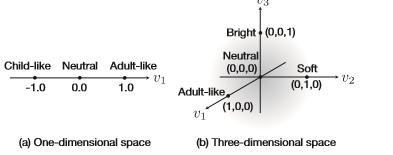
\includegraphics{exemploHMM.png}
		
		\subsubsection{Controle do Sintentisador de voz cantada baseado em MRHSMM}
		
		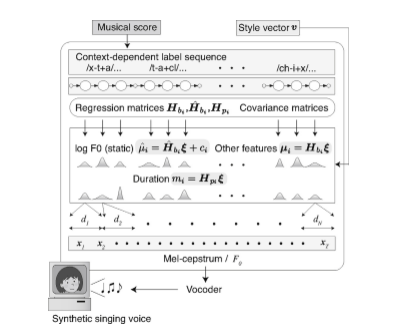
\includegraphics{esquemaHMM.png}
		
		Durante a fase de síntese o usuário do programa adiciona vetores de estilos de acorodo com a intenção e a expressividade pretendida.
		Parametros de output como duração são gerados pelos vetores de estilos dados e matrizes de regressões treinadas usando MRHSMMs
		
		Resultado de todo esse processo é um sequência HSMM usando parametros de geração de fala
		
		MRHSMM possui uma dificuldade de gerar contorno F0 que acompanhe o contexto de mudança de altura das notas o author TAKASHI NOSE, propõe um treinamento de HSMM e HMM nos parametros 
		
	
	\subsection{FrameWorks Sintetisador de Voz}
	
		Frame Work de um Sistema Sintetisador de Voz:
		
		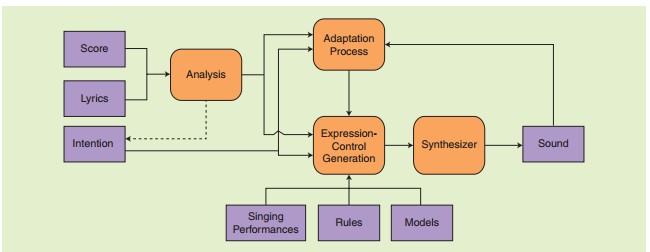
\includegraphics{frameWork.png}
		
		\subsubsection{Input}
		Consiste da partitura, letra e emoção.
		o input é analisado e derivado em uma transcrição fonética, alinhamento com a performance alvo ou dados contextuais.\cite{FrameWork}\linebreak
		
		\subsubsection{Expressão}
		Expressão músical é um conceito intuitivo porém dificil de se definir. A expressão é chave na percepção da qualidade e naturalidade musical.
		No caso da voz cantada implica-se usar vários outros parametro além de frequencia e amplitude. Psicológicamente contorno do timbre, vibrato, tremolo, timing fonético.\cite{FrameWork}\linebreak
	
	
	\subsection{Envoltoria F0}
	
	Envoltórias F0 são usadas para expressar informação linguistica, para-linguística e não-linguistica.\cite{SaitouF0}
	\linebreak
	
	As Envoltória F0 apresentam três (3) características importantes que fazem diferenciar uma voz falada a uma voz cantada.\cite{SaitouNada}
	\linebreak
	\begin{itemize}
		\item 1 - O alcance dinâmico de uma envoltória F0 é mais largo que o de uma voz falada
		\item 2 - A envoltória F0 corresponde e tende a se manter estável em uma nota. A mudança de nota de uma envoltória F0 corresponde a melodia da música
		\item 3 - Existem muita flutuações f0 que são apenas observadas em apenas vozes cantadas
	\end{itemize}
	
	
	\subsection{Sintese de Voz em Mandarím}
		Utiliza-se a técnica HNM para a sintese da voz cantada em mandarím. HNM significa , "harmonic plus noise model".
		O modelo HNM divide o espectro de um sinal em dois(2) com larguras não iguais para modelagem melhor do espectro.\cite{LinRobos}
	

 

\section{Sistema Auditivo}
	\subsection{Introdução}
	O Sistema auditivo consiste em componentes periféricos e centrais.Atualmente a maior parte do conhecimento do funcionamento dos sistemas auditivos deriva de estudos de animais não humanos.\cite{Foundation1} 
	
	Sistema auditivo diferencia-se entre espécies em jeitos interessantes.
	Por exemplo algumas espécies tem caracteristicas diferentes relacionadas aos sinais vocais mais utilizados por ela mesma.\cite{Foundation1}
	
	\subsection{Intensidade}
	Como a frequência de um estímulo a intensidade dele é processado e codificado sub-cortical nos dois lados do cérebro em todos os níveis no cerébro.\cite{Foundation1}
		


\section{Voz e Propriedades Linguísticas}
	Uma divisão importante de acordo com Flanagen, são as letras separados em classificações Vogais e Consoantes que se associam a um movimento do trato vocal correspondente~\cite{JFlanagan}.
	
	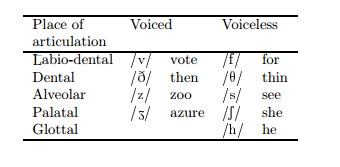
\includegraphics{tabelaConsoantes.png}
	
	\subsection{Vogais}
	
	O trato vocal ao produzir uma vocal, em um articação normal, mantém-se relativamente estável.Há uma opção de contribuição das cavidades nasais, uma cobertura porém é negligenciável.Baseado nessas caracteristicas é divididos todas as consonantes. A tabela abaixo explica:
	
	
	\subsection{Consoantes}
	Sons produzidos com constrições em algum ponto no trato vocal. Dividido em quatro (4) classes, baseados em duas funcionalidades binárias, sonorant e continuant.
	
	
		\subsubsection{Sonorant}	 
			Sonorant pode ser traduzido como "cantado". Consoantes Sonorant são sons que não aumentam a pressão do ar dentro do trato vocal pois a constrição não é muito justa ou o palato continua aberto, deixando ar escapar por ele.
			
		\subsubsection{Continuant}
			Uma consoante discontinuant é produzida por um fechamento completo em algum ponto no trato vocal.



\postextual

\bibliographystyle{plain}

\bibliography{bibliografia}


\end{document}


